\documentclass[11pt,a4paper]{article}
\usepackage[T1]{fontenc}
\usepackage[margin=2.3cm]{geometry}
\usepackage{amsmath,amssymb}
\usepackage{graphicx}
\usepackage[dvipsnames]{xcolor}
\usepackage{enumitem}
\usepackage[colorlinks=true,linkcolor=blue,urlcolor=blue]{hyperref}
\setlength{\parskip}{0.6em}
\setlength{\parindent}{0pt}
\begin{document}

\begin{center}{\LARGE\bfseries openfridge}\\[0.4em]{\large Explain and size the fridge that keeps your food cold, in three sessions.}\\[0.2em]\small PAN IIT OSS explainer \textbullet{} middle school to higher secondary (levels 2-4)\end{center}

\section*{Why this exists}
Every kitchen has a machine that moves heat uphill, from a cold box into a warm room. This explainer shows the mathematics behind that: an energy balance, the coefficient of performance and the Carnot limit, and a simplified cycle you can build yourself.

\section*{The end goal}
Explain and size the refrigerator cycle that keeps food cold. The end goal is to explain and size the refrigerator cycle that keeps food cold. The same ideas carry over to air conditioners and heat pumps, which run the same cycle for different purposes.

\section*{How the three sessions build up}
\begin{enumerate}[nosep]
\item \textbf{Session 1: Why a fridge needs electricity: the four parts and the energy balance} (Level 1, conceptual interactive model, 60 min).
\item \textbf{Session 2: COP, the Carnot limit and sizing a fridge for a heat leak} (Level 2, mathematical engineering model, 75 min).
\item \textbf{Session 3: A vapour-compression cycle, validated, and the energy bill} (Level 3, simulation and validation, 90 min).
\end{enumerate}

\section{Session 1: Why a fridge needs electricity: the four parts and the energy balance}

\subsection*{A. Real-world problem}
Leave a warm drink on a table and it cools to room temperature on its own: heat flows from warm to cold. A refrigerator keeps its inside colder than the kitchen, so heat must move the other way. Why does the fridge have to be plugged in, and where does the heat go? (Touch the back or side of a fridge: it is warm.)

\subsection*{B. Concept and theory}
A refrigerator is a loop of fluid with four parts. The evaporator, inside the food space, lets the fluid boil at low pressure and low temperature, so it takes heat Q\_cold from the inside. The compressor squeezes the vapour to high pressure and heats it, using electric work W. The condenser, at the back, gives heat Q\_hot to the kitchen as the hot vapour turns back to liquid. The expansion valve drops the pressure so the liquid becomes cold again. Over one full turn the fluid returns to where it started, so it stores no energy: Q\_hot = Q\_cold + W. Heat does not flow from cold to warm by itself (the second law, in Clausius's form); the compressor work is what pays for moving it. The COP is the heat removed per unit of work, COP = Q\_cold / W. It can exceed 1 because the fridge moves heat; it does not create it.

\begin{itemize}[nosep]
\item Q\_cold: heat taken from the cold inside per cycle (kJ)
\item W: work put in by the compressor per cycle (kJ)
\item Q\_hot: heat given to the warm kitchen per cycle (kJ)
\item COP: coefficient of performance, Q\_cold / W (no unit)
\item UA: wall leakiness: leak power per kelvin of temperature difference (W/K)
\end{itemize}

\begin{equation*}
Q_{\mathrm{hot}}=Q_{\mathrm{cold}}+W
\end{equation*}

\begin{equation*}
\mathrm{COP}=\frac{Q_{\mathrm{cold}}}{W}
\end{equation*}

\begin{equation*}
Q_{\mathrm{cold}}=\mathrm{COP}\times W,\qquad Q_{\mathrm{hot}}=(\mathrm{COP}+1)\,W
\end{equation*}

\begin{equation*}
P_{\mathrm{leak}}=UA\,(T_{\mathrm{room}}-T_{\mathrm{inside}})
\end{equation*}

\begin{center}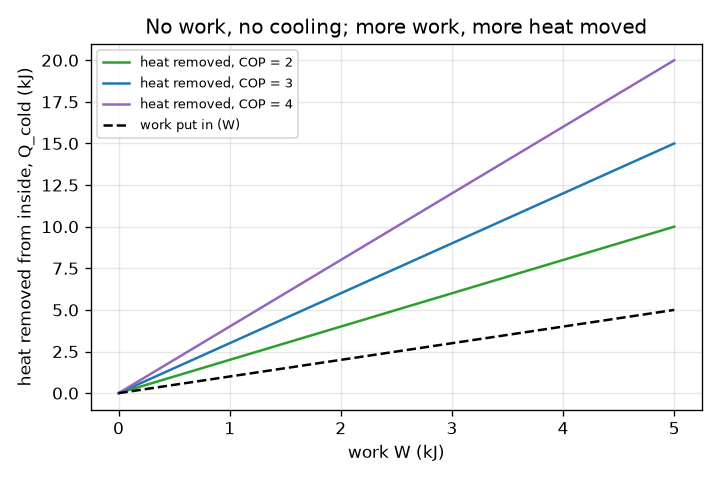
\includegraphics[width=0.85\linewidth]{figures/s01_cooling_vs_work.png}\\\small Heat removed against work for three COP values: the slope is the COP, and zero work moves nothing.\end{center}

\subsection*{E. Worked example}
A fridge takes 300 J from the inside in one cycle and uses 100 J of work. How much heat does it give to the kitchen, and what is its COP? Then: walls with UA = 2.0 W/K, a 25 C kitchen and 4 C inside; how much heat must a fridge remove every second?
\begin{enumerate}[nosep]
\item Energy balance: Q\_hot = Q\_cold + W = 300 + 100 = 400 J.
\item COP = Q\_cold / W = 300 / 100 = 3.
\item Check the direction: more heat leaves (400 J) than enters from the inside (300 J); the extra 100 J is the work.
\item Leak power = UA x (T\_room - T\_inside) = 2.0 x (25 - 4) = 2.0 x 21 = 42 W, so the fridge must remove 42 J every second.
\end{enumerate}
\textbf{Answer.} Q\_hot = 400 J and COP = 3. The walls leak 42 W, which the fridge must remove to hold 4 C.

\subsection*{F. Questions}
\begin{enumerate}[nosep]
\item \textbf{Conceptual.} Why can a refrigerator move heat from a cold interior to a warmer room only when energy is supplied? Why does the room get warmer, not colder, if you leave a fridge door open in a closed kitchen?
\item \textbf{Numerical.} A fridge takes 450 J from the inside using 150 J of work. Find Q\_hot and the COP, with units and a sanity check.
\item \textbf{Graph and simulation interpretation.} In the graph of heat removed against work, what does the slope of each line mean? What is the heat removed at W = 2 kJ for COP = 3, and at W = 0?
\item \textbf{Design and optimisation challenge.} Design: the walls leak 42 W (UA = 2.0 W/K, 25 C kitchen, 4 C inside). You can choose a fridge with COP 2.5 or COP 3.5, and your supply allows at most 15 W for the compressor. Which choices work, what is the compressor power for each, and how much heat does each give to the kitchen?
\end{enumerate}

\section{Session 2: COP, the Carnot limit and sizing a fridge for a heat leak}

\subsection*{A. Real-world problem}
A kitchen fridge holds 4 C inside while the kitchen is 25 C, and heat leaks in through the walls all day. How much electric power must the compressor use? Why does the same fridge use more power in a hot summer kitchen? And is there a best possible fridge, so that no company could ever beat it?

\subsection*{B. Concept and theory}
The best possible COP depends only on the two temperatures, measured in kelvin: T(K) = T(C) + 273.15. A reversible fridge working between a cold space at T\_c and a warm room at T\_h has COP\_Carnot = T\_c / (T\_h - T\_c). Any real fridge is below this limit; we write COP = eta2 x COP\_Carnot, where eta2 (between 0 and 1) collects all real losses. In steady state the fridge removes exactly the heat that leaks in, Q\_cold = leak, so the compressor power is W = Q\_cold / COP, and the kitchen receives Q\_hot = Q\_cold + W. A smaller temperature difference T\_h - T\_c means a larger COP, so a hot kitchen or a colder inside needs more power. The limit follows from the second law: a cycle that beat it would make the total entropy of the fridge and its surroundings decrease.

\begin{itemize}[nosep]
\item T\_c: temperature of the cold space (inside) (K)
\item T\_h: temperature of the warm room (kitchen) (K)
\item COP\_Carnot: best possible COP between T\_c and T\_h (no unit)
\item eta2: fraction of the Carnot COP actually reached (no unit)
\item Q\_cold: heat removed per second (equal to the leak in steady state) (W)
\item W: electric power used by the compressor (W)
\item Q\_hot: heat given to the kitchen per second (W)
\end{itemize}

\begin{equation*}
T(\mathrm{K})=T(^{\circ}\mathrm{C})+273.15
\end{equation*}

\begin{equation*}
\mathrm{COP}_{\mathrm{Carnot}}=\frac{T_c}{T_h-T_c},\qquad \mathrm{COP}=\eta_2\,\mathrm{COP}_{\mathrm{Carnot}}
\end{equation*}

\begin{equation*}
W=\frac{Q_{\mathrm{cold}}}{\mathrm{COP}},\qquad Q_{\mathrm{hot}}=Q_{\mathrm{cold}}+W
\end{equation*}

\begin{equation*}
T_h=T_c+\eta_2\,T_c\,\frac{W}{Q_{\mathrm{cold}}}
\end{equation*}

\begin{center}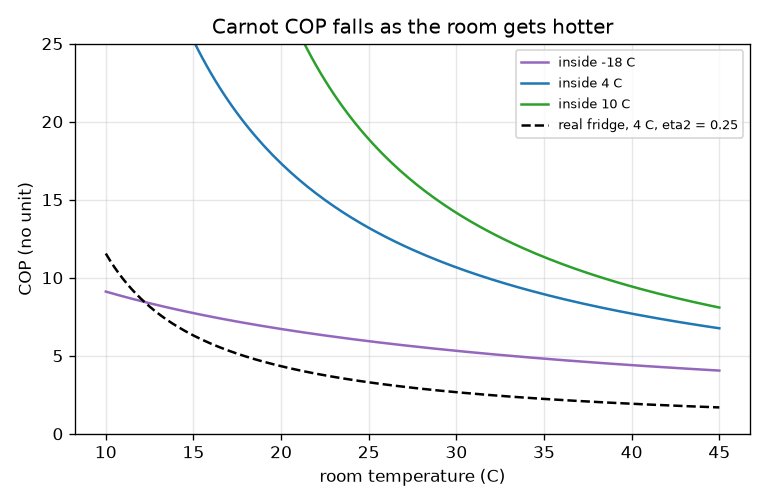
\includegraphics[width=0.85\linewidth]{figures/s02_cop_vs_room.png}\\\small Carnot COP against room temperature for three inside temperatures, with a real fridge (eta2 = 0.25) dashed.\end{center}

\subsection*{E. Worked example}
A fridge holds 4 C in a 25 C kitchen. The heat leak is 60 W and eta2 = 0.25. Find the Carnot COP, the real COP, the compressor power and the heat given to the kitchen.
\begin{enumerate}[nosep]
\item Convert: T\_c = 4 + 273.15 = 277.15 K and T\_h = 25 + 273.15 = 298.15 K, so T\_h - T\_c = 21 K.
\item COP\_Carnot = 277.15 / 21 = 13.20.
\item COP = 0.25 x 13.20 = 3.30.
\item W = Q\_cold / COP = 60 / 3.30 = 18.2 W.
\item Q\_hot = 60 + 18.2 = 78.2 W. Check: Q\_hot / W is 4.3 = COP + 1.
\end{enumerate}
\textbf{Answer.} Carnot COP 13.20, real COP 3.30, compressor power 18.2 W, heat to the kitchen 78.2 W.

\subsection*{F. Questions}
\begin{enumerate}[nosep]
\item \textbf{Conceptual.} Why can no fridge have a COP above the Carnot value? And why does a freezer at -18 C have a lower Carnot COP than a fridge at 4 C in the same kitchen?
\item \textbf{Numerical.} A fridge holds 5 C in a 30 C kitchen with a 40 W heat leak and eta2 = 0.30. Find the Carnot COP, the real COP, the compressor power and Q\_hot.
\item \textbf{Graph and simulation interpretation.} On the COP graph for a 4 C inside, estimate by what fraction the Carnot COP falls when the kitchen goes from 25 C to 35 C. Confirm with the formula.
\item \textbf{Design and optimisation challenge.} Design: the heat leak is 60 W, the inside is 4 C and the compressor power must not exceed 15 W. Find the warmest kitchen allowed if eta2 = 0.30. Then, for a 32 C kitchen, find the least eta2 that meets the limit. State the trade-off.
\end{enumerate}

\section{Session 3: A vapour-compression cycle, validated, and the energy bill}

\subsection*{A. Real-world problem}
Session 2 assumed that a real fridge reaches a fraction eta2 of the Carnot COP. Where does that fraction come from? In a real fridge the fluid must be colder than the food to take its heat and hotter than the kitchen to give heat to it, and the compressor is not perfect. How much does that cost, how does the COP change when the kitchen gets hot, and what does a fridge cost to run in a year? Note: the working fluid here is a toy refrigerant with illustrative numbers, not any real refrigerant.

\subsection*{B. Concept and theory}
The cycle has four states. State 1: saturated vapour leaves the evaporator at T\_evap. Compression to the condenser pressure is ideally isentropic (state 2s); for an ideal-gas vapour T\_2s = T\_1 (P\_cond / P\_evap)\textasciicircum{}(R / cp). A real compressor with isentropic efficiency eta\_c needs more work: h\_2 = h\_1 + (h\_2s - h\_1) / eta\_c. State 3: saturated liquid leaves the condenser at T\_cond. The expansion valve does no work and exchanges no heat, so h\_4 = h\_3 and the liquid partly flashes to vapour. The toy fluid uses the same cp for liquid and vapour and a constant latent heat L, which makes P\_sat follow the Clausius-Clapeyron relation exactly. Per kilogram of fluid: q\_evap = h\_1 - h\_4, work = h\_2 - h\_1, q\_cond = h\_2 - h\_3, and COP = q\_evap / work. For the whole fridge the evaporator is dt\_ev colder than the inside and the condenser dt\_cd hotter than the kitchen; then eta2 = COP / COP\_Carnot(inside, kitchen) is a result. Validation: q\_cond = q\_evap + work; state 2s has the same entropy as state 1; the COP stays below the Carnot value; and entropy is generated. Energy per year follows from the load (walls plus door openings), the duty cycle d = load / capacity and the electric power while running, capacity / COP.

\begin{itemize}[nosep]
\item T\_evap, T\_cond: evaporator and condenser temperatures of the refrigerant (C)
\item P\_sat: saturation pressure (bar)
\item h: specific enthalpy (zero for liquid at 0 C) (kJ/kg)
\item cp, L, R: toy fluid: specific heat 0.8, latent heat 300, gas constant 0.10 (kJ/(kg K), kJ/kg, kJ/(kg K))
\item eta\_c: compressor isentropic efficiency (no unit)
\item q\_evap, work, q\_cond: heat taken, work and heat given per kg of fluid (kJ/kg)
\item d: duty cycle: fraction of time the compressor runs (no unit)
\item E: energy per year (kWh)
\end{itemize}

\begin{equation*}
P_{\mathrm{sat}}(T)=P_0\exp\!\left[-\frac{L}{R}\left(\frac1T-\frac1{T_0}\right)\right]
\end{equation*}

\begin{equation*}
T_{2s}=T_1\left(\frac{P_{\mathrm{cond}}}{P_{\mathrm{evap}}}\right)^{R/c_p},\qquad h_2=h_1+\frac{h_{2s}-h_1}{\eta_c}
\end{equation*}

\begin{equation*}
h_4=h_3,\qquad \mathrm{COP}=\frac{h_1-h_4}{h_2-h_1}
\end{equation*}

\begin{equation*}
q_{\mathrm{cond}}=q_{\mathrm{evap}}+w,\qquad \mathrm{COP}\le\frac{T_{\mathrm{evap}}}{T_{\mathrm{cond}}-T_{\mathrm{evap}}}
\end{equation*}

\begin{equation*}
E=\left(d\,\frac{\dot Q_{\mathrm{cap}}}{\mathrm{COP}}+P_{\mathrm{overhead}}\right)\times 8760\ \mathrm{h},\qquad d=\frac{UA\,\Delta T+\dot Q_{\mathrm{door}}}{\dot Q_{\mathrm{cap}}}
\end{equation*}

\begin{center}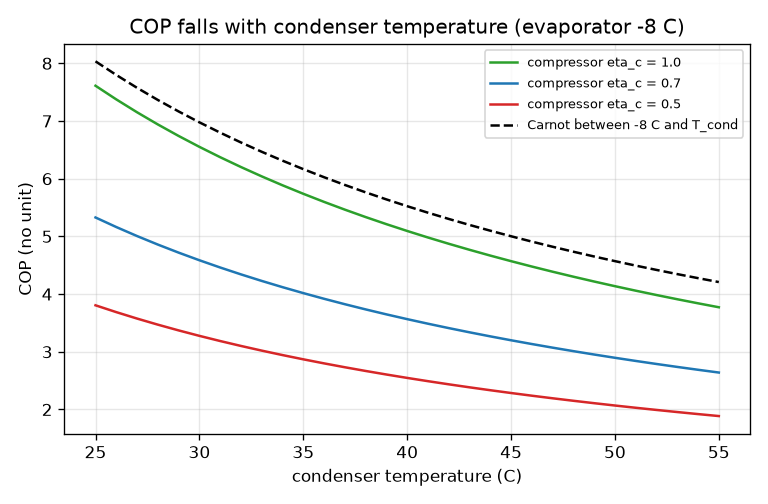
\includegraphics[width=0.85\linewidth]{figures/s03_cop_vs_condenser.png}\\\small COP against condenser temperature for three compressor efficiencies, below the Carnot limit.\end{center}

\subsection*{E. Worked example}
Evaporator at -8 C, condenser at 35 C, compressor efficiency 0.7. Find the pressures, the work, the heat taken per kilogram and the COP, and check the energy balance.
\begin{enumerate}[nosep]
\item Pressures: P\_evap = 2.08 bar and P\_cond = 10.10 bar, so the pressure ratio is 4.85.
\item h\_1 = 0.8 x (-8) + 300 = 293.6 kJ/kg and h\_3 = 0.8 x 35 = 28.0 kJ/kg, with h\_4 = h\_3 = 28.0.
\item q\_evap = h\_1 - h\_4 = 293.6 - 28.0 = 265.6 kJ/kg.
\item T\_2s = 265.15 x 4.85\textasciicircum{}0.125 = 265.15 x 1.218 = 323.0 K, which is 49.8 C; the ideal work is 0.8 x (323.0 - 265.15) = 46.3 kJ/kg.
\item Real work = 46.3 / 0.7 = 66.1 kJ/kg, so COP = 265.6 / 66.1 = 4.02.
\item q\_cond = h\_2 - h\_3 = 359.7 - 28.0 = 331.7 kJ/kg, and q\_evap + work = 265.6 + 66.1 = 331.7. The energy balance closes.
\item Carnot between -8 C and 35 C: 265.15 / 43 = 6.17, and 4.02 is below it, as it must be.
\end{enumerate}
\textbf{Answer.} P\_evap 2.08 bar, P\_cond 10.10 bar, work 66.1 kJ/kg, q\_evap 265.6 kJ/kg, COP 4.02 (below the Carnot value 6.17). For a whole fridge holding 4 C in a 25 C kitchen the same cycle (evaporator -4 C, condenser 35 C) gives COP 4.53, which is 0.34 of the Carnot COP 13.20: the fraction eta2 of Session 2 is now a result.

\subsection*{F. Questions}
\begin{enumerate}[nosep]
\item \textbf{Conceptual.} Why does the COP of the cycle fall when the condenser temperature rises, even though nothing else changes? Why is the cycle COP always below the Carnot COP?
\item \textbf{Numerical.} For the cycle in the worked example, find the COP if the compressor efficiency is 0.5 instead of 0.7. Show how the result follows from the isentropic work.
\item \textbf{Graph and simulation interpretation.} On the COP graph (evaporator -8 C, eta\_c = 0.7) read the COP at condenser temperatures of 25 C and 45 C. How large is the fall, and how far below the Carnot line is the cycle?
\item \textbf{Design and optimisation challenge.} Design: with capacity 150 W, UA = 3.0 W/K, 4 C inside, 30 door openings a day and compressor efficiency 0.7, find the warmest whole-degree kitchen for which the compressor runs at most 60 percent of the time. Then say what happens at 34 C and what you could change.
\end{enumerate}

\section{Real-world mini-project}
\textbf{Estimate the energy bill of a kitchen fridge.} A household in a hot city wants a rough idea of what its fridge costs to run, and whether the compressor has enough margin. Use \texttt{fridge\_year} from Session 3 (wall leak UA = 3.0 W/K, 4 C inside, cooling capacity 150 W, compressor efficiency 0.7, 5 W of fans and lights, 30 door openings a day). General education only; the tariff of 8 per kWh is an illustration, not advice. Estimate the yearly energy and cost for kitchens at 22, 28 and 34 C, then find the warmest whole-degree kitchen for which the compressor runs no more than 60 percent of the time.

\section{The path ahead}
\begin{enumerate}[nosep]
\item \textbf{Session 4: Replace the toy fluid by real property data.} A property function built from a published table for one real refrigerant, used in the same cycle code.
\item \textbf{Session 5: Superheat and subcooling.} Extend the cycle with two extra temperature offsets and show the effect on the P-h loop.
\item \textbf{Session 6: Size the heat exchangers.} Replace the fixed offsets of 8 K and 10 K by values found from UA values with an iterative solution.
\item \textbf{Session 7: Thermostat cycling over a day.} A time-stepping simulation of the inside temperature with a thermostat and a thermal mass.
\item \textbf{Session 8: Moisture and door openings.} An improved door-load model with humid air.
\end{enumerate}

\section{Answers and hints}

\subsection*{Session 1}
\begin{enumerate}[nosep]
\item \textbf{Conceptual.} Hint: Think about which way heat flows by itself, and use Q\_hot = Q\_cold + W. Solution: Heat flows by itself only from warm to cold; moving it the other way is not spontaneous, so something must pay for it, and the compressor's electrical work W does. The energy balance Q\_hot = Q\_cold + W shows that the kitchen receives all the heat taken from the inside plus the work. With the door open in a closed kitchen the fridge takes heat from the kitchen air and gives back more (Q\_cold + W), so the net effect on the room is the work W: it warms the kitchen a little, it never cools it.
\item \textbf{Numerical.} Hint: Q\_hot = Q\_cold + W and COP = Q\_cold / W. Solution: Q\_hot = 450 + 150 = 600 J. COP = 450 / 150 = 3 (no unit). Sanity check: Q\_hot is larger than Q\_cold, and the COP is positive; the difference Q\_hot - Q\_cold equals the work 150 J.
\item \textbf{Graph and simulation interpretation.} Hint: Read the line for COP = 3 at W = 2, and look at where each line starts. Solution: The slope is Q\_cold / W, which is the COP. At W = 2 kJ and COP = 3 the heat removed is 6 kJ. At W = 0 every line gives 0: with no work nothing is moved. A steeper line means a better fridge, because it moves more heat for each kJ of work.
\item \textbf{Design and optimisation challenge.} Hint: In steady state Q\_cold = 42 W, so W = Q\_cold / COP and Q\_hot = Q\_cold + W. Solution: COP 2.5: W = 42 / 2.5 = 16.8 W, which is above the 15 W limit, so it does not work. COP 3.5: W = 42 / 3.5 = 12.0 W, which works. Heat to the kitchen for the COP 3.5 fridge: 42 + 12 = 54 W (for COP 2.5 it would be 58.8 W). Trade-off: a higher COP costs more to build; assumption: steady state and a constant COP.
\end{enumerate}

\subsection*{Session 2}
\begin{enumerate}[nosep]
\item \textbf{Conceptual.} Hint: Look at the formula T\_c / (T\_h - T\_c) and ask what happens to the numerator and the denominator. Solution: A fridge with a higher COP would take heat from the cold space and give it to the room with less work than the best reversible cycle, which would make the total entropy of the fridge and surroundings decrease; the second law forbids it. For the freezer, the temperature difference is larger (43 K instead of 21 K) and T\_c is smaller, so T\_c / (T\_h - T\_c) is much smaller: 255.15 / 43 = 5.93 against 13.20.
\item \textbf{Numerical.} Hint: Use kelvin: T\_c = 278.15 K, T\_h = 303.15 K. Solution: T\_h - T\_c = 25 K. COP\_Carnot = 278.15 / 25 = 11.13. COP = 0.30 x 11.13 = 3.34. W = 40 / 3.34 = 12.0 W. Q\_hot = 40 + 12.0 = 52.0 W. Sanity check: W is smaller than Q\_cold, and Q\_hot is larger than both.
\item \textbf{Graph and simulation interpretation.} Hint: Read the curve at 25 C and at 35 C and take the ratio; the formula ratio is 21 / 31. Solution: The curve reads about 13.2 at 25 C and about 8.9 at 35 C. The ratio is 8.94 / 13.20 = 0.68, so the COP falls by about a third. The formula gives the same ratio, (T\_h - T\_c) at 25 C divided by that at 35 C, 21 / 31 = 0.68. The same fridge therefore needs about 1.5 times the power in the hotter kitchen.
\item \textbf{Design and optimisation challenge.} Hint: Use T\_h = T\_c + eta2 T\_c W / Q\_cold for the first part, and COP = Q\_cold / W for the second. Solution: First part: T\_h = 277.15 + 0.30 x 277.15 x 15 / 60 = 277.15 + 20.79 = 297.94 K, which is 24.8 C. Second part: at 32 C, COP\_Carnot = 277.15 / 28 = 9.90; the needed COP is 60 / 15 = 4, so eta2 must be at least 4 / 9.90 = 0.404. With eta2 = 0.30 the power would be 20.2 W, too high. Trade-off: a higher eta2 needs a better compressor and larger heat exchangers (higher cost), while a smaller leak (more insulation) lowers the power for the same fridge. Assumption: steady state and a constant eta2.
\end{enumerate}

\subsection*{Session 3}
\begin{enumerate}[nosep]
\item \textbf{Conceptual.} Hint: Look at the pressure ratio and the length of the compression 1 to 2 on the P-h diagram. Solution: A hotter condenser means a higher condenser pressure, a larger pressure ratio and a longer horizontal stretch from 1 to 2: the work rises, while the heat taken from the food (h\_1 - h\_4) even falls because h\_3 is larger. COP = q\_evap / work therefore falls. The cycle is below Carnot because the compressor is not isentropic, the valve wastes the expansion work and the heat exchange happens across finite temperature differences, all of which generate entropy; the checkpoint verifies that the entropy generated is positive.
\item \textbf{Numerical.} Hint: work = ideal work / eta\_c, so COP is proportional to eta\_c. Solution: The ideal work is 46.3 kJ/kg, so the real work is 46.3 / 0.5 = 92.6 kJ/kg. q\_evap is unchanged at 265.6 kJ/kg, so COP = 265.6 / 92.6 = 2.87. Check: 4.02 x 0.5 / 0.7 = 2.87. Units: COP has no unit; work and heat in kJ/kg.
\item \textbf{Graph and simulation interpretation.} Hint: Read the blue curve and the grey Carnot curve at each condenser temperature. Solution: The cycle gives COP 5.33 at 25 C and 3.20 at 45 C, a fall of 40 percent. The Carnot values are 265.15 / 33 = 8.04 and 265.15 / 53 = 5.00, so the cycle reaches about 66 percent and 64 percent of Carnot between the two evaporator and condenser temperatures. A hot kitchen costs about 40 percent of the COP for 20 K more condenser temperature.
\item \textbf{Design and optimisation challenge.} Hint: Use fridge\_year(t\_room)['duty'] for each whole-degree room temperature. Solution: The duty is 0.592 at 33 C and 0.613 at 34 C, so the warmest kitchen is 33 C. At 34 C the compressor runs 61 percent of the time and uses about 266 kWh a year against 254 kWh at 33 C. To bring the duty down you can reduce the load (better insulation lowers UA, fewer door openings) or raise the capacity (a bigger compressor), but a bigger compressor starts and stops more often and costs more. Assumptions: steady load, sensible door load only.
\end{enumerate}

\section{How to join}
Read \texttt{CONTRIBUTING.md} in the repository, then pick an issue labelled \texttt{good first issue}. Repository: \url{https://github.com/KrunalPanchal1995/openfridge}

\end{document}
